%%%%%%%%%%%%%%%%%%%%%%%%%%%%%%%%%%%%%%%%%%%%%%%%%%%%%%%%
%%
\chapter{Installation}
\label{chapter:installation}
%%
%%%%%%%%%%%%%%%%%%%%%%%%%%%%%%%%%%%%%%%%%%%%%%%%%%%%%%%%


%%%%%%%%%%%%%%%%%%%%%%%%%%%%%%%%%%%%%%%%%%%%%%%%%%%%%%%%
%%
\section{Introduction}
\label{ch:install:installintro}
%%
%%%%%%%%%%%%%%%%%%%%%%%%%%%%%%%%%%%%%%%%%%%%%%%%%%%%%%%%

Once finalized the installation should just be a download, run set-up.py and configure the DRS directories, however, during development the following stages are required.

\DevNote{Currently the download repository on git-hub is private and requires a git-hub account, and the user to be added to the list of collaborators. To be added to the collaborators please email \url{neil.james.cook@gmail.com} with your git-hub user name.}







%%%%%%%%%%%%%%%%%%%%%%%%%%%%%%%%%%%%%%%%%%%%%%%%%%%%%%%%
%%
\section{Download}
\label{ch:install:installDownload}
%%
%%%%%%%%%%%%%%%%%%%%%%%%%%%%%%%%%%%%%%%%%%%%%%%%%%%%%%%%

Get the latest version of the DRS (for \instrument version \MyCodeVersion). Use any of the following ways:

\begin{itemize}
\item manually download from here: \url{\DRSLatestURL}

\item use Git:
\begin{cmdbox}
git checkout (*\DRSGitURL*)
\end{cmdbox}

\item use SVN:
\begin{cmdbox}
svn checkout  (*\DRSGitURL*)
\end{cmdbox}

\item use ssh:
\begin{cmdbox}
scp -r (*\DRSsshURL*)
\end{cmdbox}

\end{itemize}


%%%%%%%%%%%%%%%%%%%%%%%%%%%%%%%%%%%%%%%%%%%%%%%%%%%%%%%%
%%
\clearpage
\newpage
\section{Prerequisites}
\label{ch:install:prerequisites}
%%
%%%%%%%%%%%%%%%%%%%%%%%%%%%%%%%%%%%%%%%%%%%%%%%%%%%%%%%%

It is recommended to install the latest version of Anaconda python distribution, available for Windows, \mac and Linux (here: \url{https://www.anaconda.com/download/}). However one can run the DRS on a native python installation. \\

\noindent We recommend python 3 over python 2 for long term continued support (however the latest version of the DRS supports the newest versions of python 2.7).

\begin{note}
Before installing the DRS you must have one of the following:
\begin{itemize}
\item Latest version of Anaconda (for python 2 or python 3) --- RECOMMENDED
\item An Up-to-date version of python (python 2 or python 3)
\end{itemize}
\end{note}


% -------------------------------------------------------
\subsection{Anaconda python distribution}
\label{ch:install:prerequisites:anaconda}
% -------------------------------------------------------

A valid version of the Anaconda python distribution (for python 2 or python 3)
\noindent Currently tested version of python are:
\begin{itemize}
\item Python 2.7.13 and Anaconda 4.4.0
\item Python 3.6.3 and Anaconda 5.0.1 --- RECOMMENDED
\end{itemize}



% -------------------------------------------------------
\subsection{Separate python installation}
\label{ch:install:prerequisites:separate_python}
% -------------------------------------------------------

An up-to-date version of python (either python 2 or python 3) and the following python modules (with version of python they were tested with).
\begin{itemize}
\item Python 3.6.4
	\begin{itemize}
	\item \Program{astropy} (tested with version 2.0.3)
	\item \Program{matplotlib} (tested with version 2.1.2)
	\item \Program{numpy} (tested with version 1.14.0)
	\item \Program{scipy} (tested with version 1.0.0)
	\item and the following built-in modules (comes with python): 
	\Program{\twound{future}\twound}, \Program{calender}, \Program{code}, \Program{collections}, \Program{datetime}, \Program{filecmp}, \Program{glob}, \Program{os}, \Program{pdb}, \Program{pkg\_resources}, \Program{shutil}, \Program{string}, \Program{sys}, \Program{time}, \Program{warnings}.
	\end{itemize}
\item Python 2.7.14
	\begin{itemize}
	\item astropy (tested with version 2.0.3)
	\item matplotlib (tested with version 2.1.2)
	\item numpy (tested with version 1.14.0)
	\item scipy (tested with version 1.0.0)
	\item and the following built-in modules (comes with python): 
	\Program{\twound{future}\twound}, \Program{calender}, \Program{code}, \Program{collections}, \Program{datetime}, \Program{filecmp}, \Program{glob}, \Program{os}, \Program{pdb}, \Program{pkg\_resources}, \Program{shutil}, \Program{string}, \Program{sys}, \Program{time}, \Program{warnings}.
	\end{itemize}
\end{itemize}


%%%%%%%%%%%%%%%%%%%%%%%%%%%%%%%%%%%%%%%%%%%%%%%%%%%%%%%%
%%
\clearpage
\newpage
\section{Installation Linux and macOS}
\label{ch:install:installunix}
%%
%%%%%%%%%%%%%%%%%%%%%%%%%%%%%%%%%%%%%%%%%%%%%%%%%%%%%%%%

Currently the DRS has to be installed manually. This involves the following steps:
\begin{enumerate}
\item Extraction (Section \ref{ch:install:installunix:extraction})
\item Modify environmental settings (Section \ref{ch:install:installunix:environ_settings})
\item Make recipes executable (Section \ref{ch:install:installunix:executable})
\end{enumerate}

% -------------------------------------------------------
\subsection{Extraction}
\label{ch:install:installunix:extraction}
% -------------------------------------------------------

The first step is to extract the DRS into a folder (the \InstallDIR).

\noindent Do this by using the following commands:
\begin{cmdbox}
cd (* \InstallDIR *)
unzip DRS.zip
\end{cmdbox}

% -------------------------------------------------------
\subsection{Modify environmental settings}
\label{ch:install:installunix:environ_settings}
% -------------------------------------------------------

The next step is to modify your PATH and PYTHONPATH environmental variables (to include the \InstallDIR. This depends which shell you are using (type `\lstinline[style=bashstyle]{echo $0}' to find out which).

\begin{itemize}
	\item In bash open the `.bashrc' or `.bash\_profile' text file in your home ($\sim$) directory (or create it if it doesn't exist)

	\begin{bashbox}[title={e.g. in $\sim$/.bashrc or $\sim$/.bash\_profile}]
	@export@ <PATH>=".:(*\InstallDIR*)/bin/:{(*\$*)PATH}"
	@export@ <PYTHONPATH>=".:(*\InstallDIR*):(*\InstallDIR*)/bin/:{(*\$*)PYTHONPATH}"
	\end{bashbox}

	\item In csh/tcsh open the `.cshrc' or `.tcshrc' text file in your home ($\sim$) directory (or create it if it doesn't exist).

	\begin{cshbox}[title={e.g. in $\sim$/.tcshrc}]
	@setenv@ <PATH> ".:(*\InstallDIR*)/bin/":{(*\$*){PATH}}"
	\end{cshbox}

	In csh/tcsh one has to check whether `\$PYTHONPATH' exists before adding to the PYTHONPATH. To check type:

	\begin{cmdbox}
	echo (*\$*)PYTHONPATH
	\end{cmdbox}

	\begin{itemize}
	\item \begin{thighlight}
		If the response is:
		\begin{cmdboxprint}
		PYTHONPATH: Undefined variable.
		\end{cmdboxprint}

		Then in the `.cshrc' or `.tcshrc' add: 

		\begin{cshbox}[title={e.g. in $\sim$/.tcshrc}]
		@setenv@ <PYTHONPATH> ".:(*\InstallDIR*):(*\InstallDIR*)/bin/"
		\end{cshbox}
		\end{thighlight}

	\item \begin{thighlight}
		If the response is some paths, then in the `.cshrc' or `.tcshrc' add: 

		\begin{cshbox}[title={e.g. in $\sim$/.tcshrc}]
		@setenv@ <PYTHONPATH> ".:(*\InstallDIR*):(*\InstallDIR*)/bin/:(*\$*){PYTHONPATH}"
		\end{cshbox}
		\end{thighlight}

	\end{itemize}

\end{itemize}

% -------------------------------------------------------
\subsection{Make recipes executable}
\label{ch:install:installunix:executable}
% -------------------------------------------------------

\noindent To run the recipes from the command line (without starting python) one must make them executable. Do this by using the following command:
\begin{cmdbox}
chmod +x (*\InstallDIR*)/bin/*.py
\end{cmdbox}


%%%%%%%%%%%%%%%%%%%%%%%%%%%%%%%%%%%%%%%%%%%%%%%%%%%%%%%%
%%
\clearpage
\newpage
\section{Setting up the DRS on Linux and macOS}
\label{ch:install:setup}
%%
%%%%%%%%%%%%%%%%%%%%%%%%%%%%%%%%%%%%%%%%%%%%%%%%%%%%%%%%

Before running the DRS one must set the data paths. \\

\noindent The `\configtxtfile' file is located in the \InstallDIR in the config folder.

i.e. at \InstallDIR{/config/\configtxtfile} \\

\noindent The following keywords \textbf{must} be changed (and must be a valid path):
\begin{thighlight}
\begin{table}[H]
\begin{tabular}{p{4cm} p{0.05cm} p{2.5cm} p{0.05cm} p{4.5cm}}
\definevariable{text:tdata}{TDATA}            & = & /drs/data/        & / & Define the DATA directory\\
&&&&\\
\definevariable{text:drs_root}{DRS\_ROOT}         & = & /drs/INTROOT/     & / & Define the installation directory \\
\definevariable{text:drs_data_raw}{DRS\_DATA\_RAW}     & = & /drs/data/raw     & / & Define the folder with the raw data files in \\
\definevariable{text:drs_data_reduc}{DRS\_DATA\_REDUC}   & = & /drs/data/reduced & / & Define the directory that the reduced data should be saved to/read from \\
\definevariable{text:drs_calib_db}{DRS\_CALIB\_DB}     & = & /drs/data/calibDB & / & Define the directory that the calibration files should be saved to/read from \\
\definevariable{text:drs_data_msg}{DRS\_DATA\_MSG}     & = & /drs/data/msg     & / & Define the directory that the log messages are stored in \\
\definevariable{text:drs_data_working}{DRS\_DATA\_WORKING} & = & /drs/data/tmp/    & / & Define the working directory \\
\end{tabular}
\end{table}
\end{thighlight}
\begin{note}
Some text editors (such as TextEdit on macOS) use `smart speech-marks' these characters are invalid for python and thus care must be taken when editing the configuration files. The \calvalidate recipe (Section \ref{ch:install:validating_installunix}) will check for invalid characters and show the lines which do not have valid characters (valid characters are ASCII letters, digits, punctuation and white spaces as defined by pythons `\Program{string}' module). We suggest using text editors such as \Program{sublime-text} or a python IDE such as \Program{Pycharm}.
\end{note}

\vspace{0.25cm}

\subsection{Other configuration parameters}

If one is using the DRS in the default setup one needs to make sure the following parameters are set correctly:

\begin{itemize}
	\item \definevariable{text:user_config}{USER\_CONFIG} is set to a value of 0 (or False)
	\item \definevariable{text:drs_debug}{DRS\_DEBUG} is set to a value of 0 (or False)
	\item \definevariable{text:icdp_name}{ICDP\_NAME} is set to `constants\_SPIROU.py'
\end{itemize}

\noindent The following keywords can be changed: \\
\begin{thighlight}
\begin{table}[H]
\begin{tabular}{>{\color{red}}l c r c p{5cm}}
\definevariable{text:drs_plot}{DRS\_PLOT}    & = & 1     & / & Whether to show plots \\
\definevariable{text:print_level}{PRINT\_LEVEL} & = & "all" & / & Level at which to print \\
\definevariable{text:log_level}{LOG\_LEVEL}   & = & "all" & / & Level at which to log in log file \\
\end{tabular}
\end{table}

\noindent For the `\definevariable{text:print_level}{PRINT\_LEVEL} and \definevariable{text:log_level}{LOG\_LEVEL} keywords the values are set as follows:
\begin{itemize}
	\item "all" -- prints all events
	\item "info" -- prints info, warning and error events
	\item "warning" -- prints warning and error events
	\item "error" -- print only error events
\end{itemize}
\end{thighlight}

%%%%%%%%%%%%%%%%%%%%%%%%%%%%%%%%%%%%%%%%%%%%%%%%%%%%%%%%
%%
\clearpage
\newpage
\section{Validating Installation on Linux and macOS}
\label{ch:install:validating_installunix}
%%
%%%%%%%%%%%%%%%%%%%%%%%%%%%%%%%%%%%%%%%%%%%%%%%%%%%%%%%%

\begin{note}
One must install the DRS (Section \ref{ch:install:installunix}) AND set up the DRS (Section \ref{ch:install:setup}) before validation will be successful.
\end{note}

\noindent There are four ways to run the DRS in Linux and \mac (thus four ways to verify installation was correct).

\begin{itemize}

\item To validate running from command line type:
\begin{cmdbox}
(*\calvalidate*).py
\end{cmdbox}

\item To validate running from python/ipython from the command line type:
\begin{cmdbox}
python (*\calvalidate*)
ipython (*\calvalidate*)
\end{cmdbox}

\item To validate running from ipython, open ipython and type:
\begin{pythonbox}
@run@ (*\calvalidate*).py
\end{pythonbox}

\item To validate running from import from python/ipython, open python/ipython and type:
\begin{pythonbox}
import cal_validate_spirou
cal_validate_spirou.main()
\end{pythonbox}

\end{itemize}

\noindent If validation is successful the following should appear:

\begin{cmdboxprintspecial}
@g
HH:MM:SS.S -   || *****************************************
HH:MM:SS.S -   || * SPIROU @(#) Geneva Observatory (0.0.1)
HH:MM:SS.S -   || *****************************************
HH:MM:SS.S -   ||(dir_data_raw)      DRS_DATA_RAW=/drs/data/raw
HH:MM:SS.S -   ||(dir_data_reduc)    DRS_DATA_REDUC=/drs/data/reduced
HH:MM:SS.S -   ||(dir_calib_db)      DRS_CALIB_DB=/drs/data/calibDB
HH:MM:SS.S -   ||(dir_data_msg)      DRS_DATA_MSG=/drs/data/msg
HH:MM:SS.S -   ||(print_level)       PRINT_LEVEL=all         %(error/warning/info/all)
HH:MM:SS.S -   ||(log_level)         LOG_LEVEL=all         %(error/warning/info/all)
HH:MM:SS.S -   ||(plot_graph)        DRS_PLOT=1            %(def/undef/trigger)
HH:MM:SS.S -   ||(used_date)         DRS_USED_DATE=undefined
HH:MM:SS.S -   ||(working_dir)       DRS_DATA_WORKING=/drs/data/tmp/
HH:MM:SS.S -   ||                    DRS_INTERACTIVE is not set, running on-line mode
HH:MM:SS.S -   ||
HH:MM:SS.S -   ||Validation successful. DRS installed corrected.
@g
\end{cmdboxprintspecial}




%%%%%%%%%%%%%%%%%%%%%%%%%%%%%%%%%%%%%%%%%%%%%%%%%%%%%%%%
%%
\clearpage
\newpage
\section{Installation Windows}
\label{ch:install:install_win}
%%
%%%%%%%%%%%%%%%%%%%%%%%%%%%%%%%%%%%%%%%%%%%%%%%%%%%%%%%%

This is very similar currently to the Linux/\mac installation (in the future a `.exe' file will be given).

\begin{enumerate}
\item Extract to \InstallDIR\, with your favourite unzipping software.
\item Add \InstallDIR\, to your PYTHONPATH (Section \ref{ch:install:install_win:environ_settings})
\end{enumerate}

% -------------------------------------------------------
\subsection{How to modify environmental settings in windows}
\label{ch:install:install_win:environ_settings}
% -------------------------------------------------------

This process is a little more convoluted than on Linux or \mac system.

\begin{enumerate}
\item Go to `My computer > Properties > Advanced System Settings > Environmental Variables'. Note in windows 10 you can also click the windows icon and type `Advanced System Settings' then click `Environment Variables'.


\item under system variable `Path' click edit and add:
\begin{textbox}[title={In "Environmental Variables"}]
(*\InstallDIR*);(*\InstallDIR*)\bin;
\end{textbox}

\item if under system variable `PYTHONPATH' exists click edit and add `\InstallDIR;'\, to the end.

\noindent i.e.

\begin{textbox}[title={In "Environmental Variables"}]
(*\InstallDIR*);(*\InstallDIR*)\bin;
\end{textbox}

\item if under system variables `PYTHONPATH' does not exist create a new variable called `PYTHONPATH' and add:

\begin{textbox}[title={In "Environmental Variables"}]
%PYTHONPATH%;(*\InstallDIR*);(*\InstallDIR*)\bin\;
\end{textbox}

\end{enumerate}

\noindent Figure \ref{figure:screengrabs} shows screen-grabs of the various steps above to aid in updating PATH and PYTHONPATH.
\vspace{0.25cm}
\noindent For problems/troubleshooting see here: \url{https://stackoverflow.com/questions/3701646}.

\begin{figure}
\begin{center}
\begin{minipage}[t]{.29\textwidth}
\begin{center}
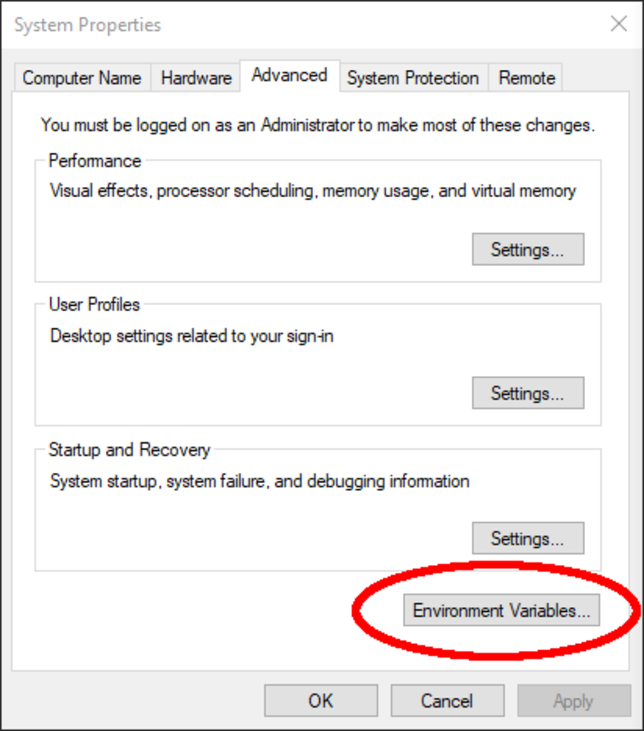
\includegraphics[width=\textwidth]{Figures/win/Win1.pdf}
(a)
\end{center}
\end{minipage}
\begin{minipage}[t]{.29\textwidth}
\begin{center}
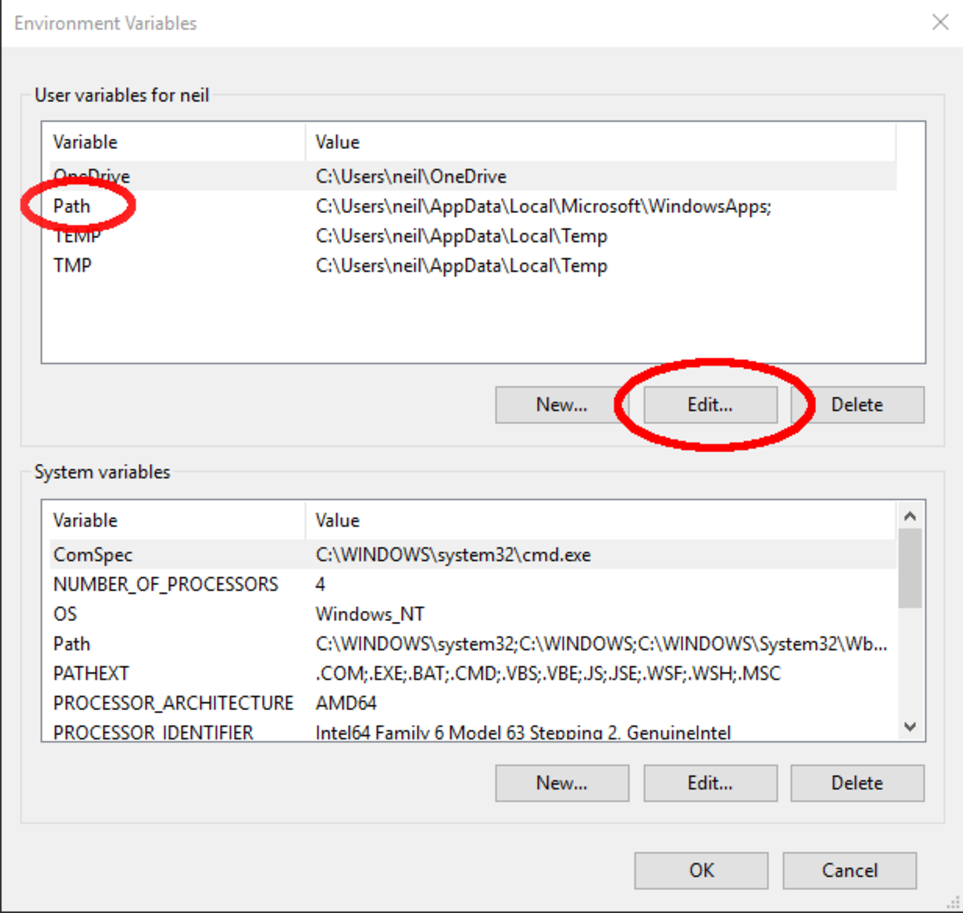
\includegraphics[width=\textwidth]{Figures/win/Win2.pdf}
(b)
\end{center}
\end{minipage}
\begin{minipage}[t]{.29\textwidth}
\begin{center}
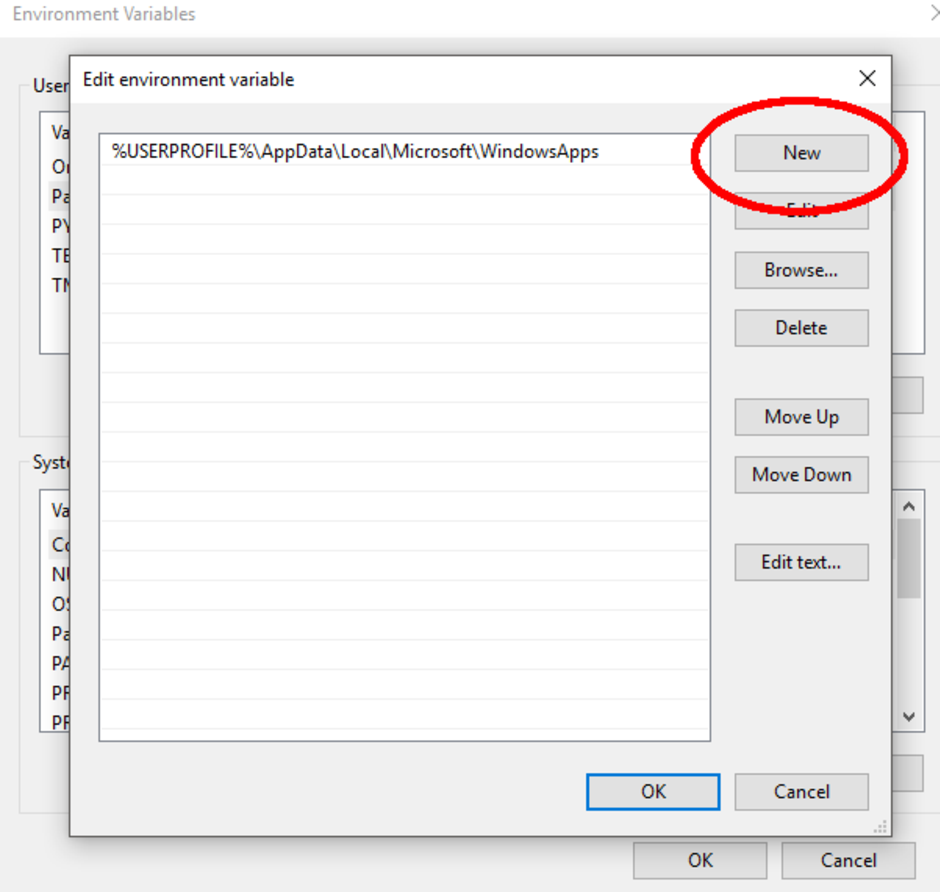
\includegraphics[width=\textwidth]{Figures/win/Win3.pdf}
(c)
\end{center}
\end{minipage}

\begin{minipage}[t]{.29\textwidth}
\begin{center}
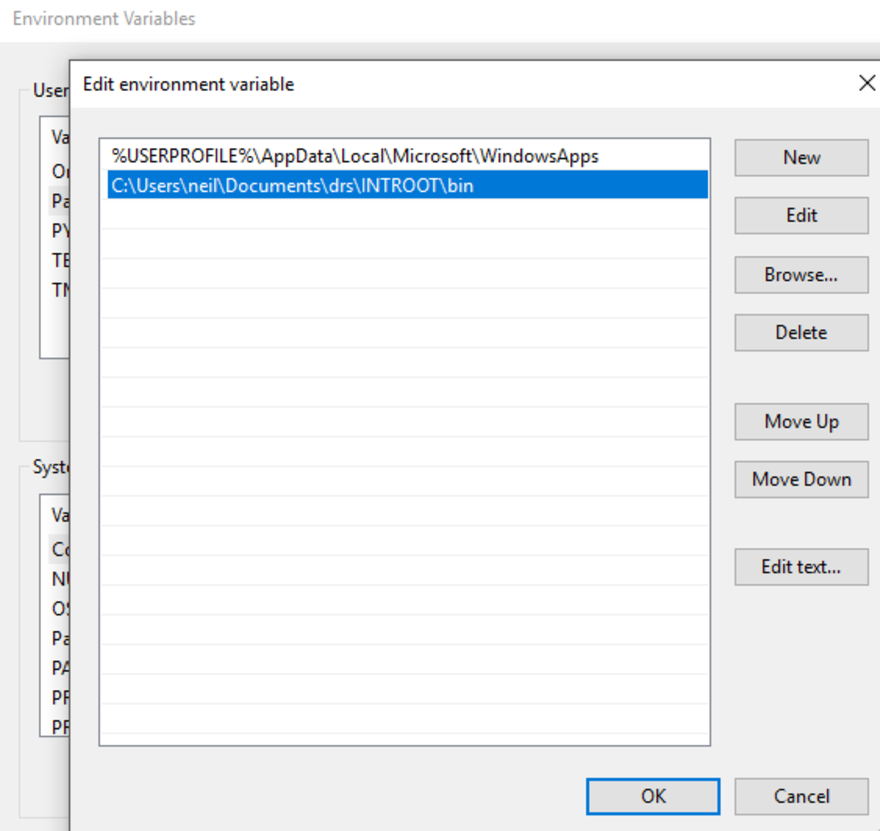
\includegraphics[width=\textwidth]{Figures/win/Win4.pdf}
(d)
\end{center}
\end{minipage}
\begin{minipage}[t]{.29\textwidth}
\begin{center}
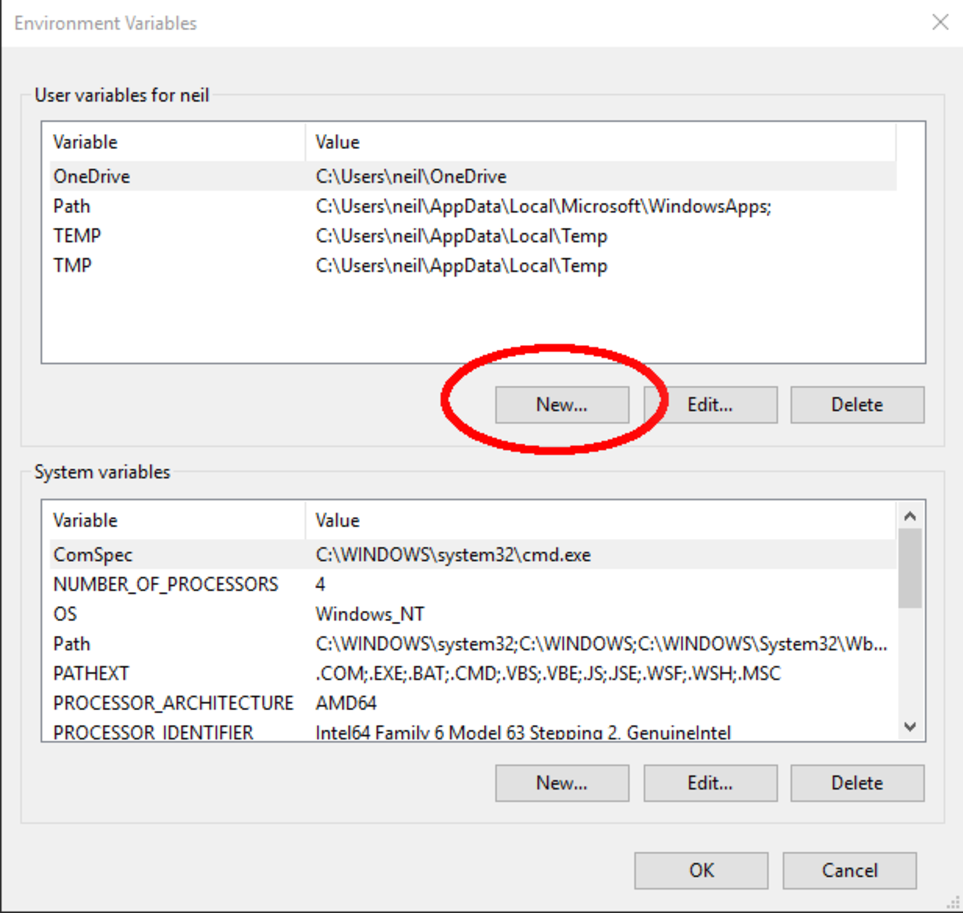
\includegraphics[width=\textwidth]{Figures/win/Win5.pdf}
(e)
\end{center}
\end{minipage}
\begin{minipage}[t]{.29\textwidth}
\begin{center}
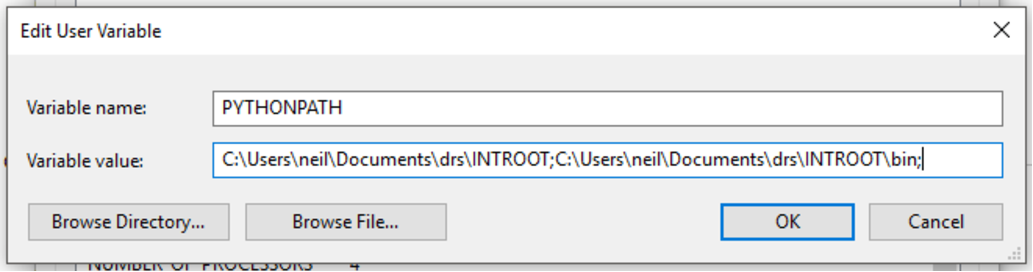
\includegraphics[width=\textwidth]{Figures/win/Win6.pdf}
(f)
\end{center}
\end{minipage}
\end{center}
\caption{(a) Once in ``Advanced system properties'' click ``Environment Variables'' (b) Click ``Path'' and click ``Edit...'' to edit the ``Path'' environmental variable (c) Once in the ``Path'' environmental variable click ``New'' to add a new path (d) Type in the new line to add variable and click ``OK'' (e) Once back in the Environmental variable page click ``New'' to add `PYTHONPATH' (f) Set the variable name to ``PYTHONPATH'' and edit the variable value accordingly. \label{figure:screengrabs} }
\end{figure}
\vspace{0.25cm}



%%%%%%%%%%%%%%%%%%%%%%%%%%%%%%%%%%%%%%%%%%%%%%%%%%%%%%%%
%%
\clearpage
\newpage
\section{Setting up the DRS (Windows)}
\label{ch:install:setup_win}
%%
%%%%%%%%%%%%%%%%%%%%%%%%%%%%%%%%%%%%%%%%%%%%%%%%%%%%%%%%

Before running the DRS one must set the data paths. \\

\noindent The `\configtxtfile' file is located in the \InstallDIR in the config folder.

i.e. at \InstallDIR\path{\\config\\}{configtxtfile} \\

\noindent The following keywords \textbf{must} be changed (and must be a valid path):
\begin{thighlight}
\begin{table}[H]
{\footnotesize
\begin{tabular}{p{4cm} p{0.05cm} p{2.5cm} p{0.05cm} p{5.5cm}}
\definevariable{text:drs_root}{TDATA}            & = & \path{C:\\Users\\User\\Documents\\drs\\data}        & / & Define the DATA directory\\
&&&&\\
\definevariable{text:drs_root}{DRS\_ROOT}         & = & \path{C:\\Users\\User\\Documents\\drs\\INTROOT}     & / & Define the installation directory \\
\definevariable{text:drs_data_raw}{DRS\_DATA\_RAW}     & = & \path{C:\\Users\\User\\Documents\\drs\\data\\raw}    & / & Define the folder with the raw data files in \\
\definevariable{text:drs_data_reduc}{DRS\_DATA\_REDUC}   & = & \path{C:\\Users\\User\\Documents\\drs\\data\\reduced} & / & Define the directory that the reduced data should be saved to/read from \\
\definevariable{text:drs_calib_db}{DRS\_CALIB\_DB}     & = & \path{C:\\Users\\User\\Documents\\drs\\data\\calibDB} & / & Define the directory that the calibration files should be saved to/read from \\
\definevariable{text:drs_data_msg}{DRS\_DATA\_MSG}     & = & \path{C:\\Users\\User\\Documents\\drs\\data\\msg}    & / & Define the directory that the log messages are stored in \\
\definevariable{text:drs_data_working}{DRS\_DATA\_WORKING} & = & \path{C:\\Users\\User\\Documents\\drs\\data\\tmp}    & / & Define the working directory \\
\end{tabular}
}
\end{table}
\end{thighlight}
\begin{note}
Note: On windows paths in windows must have a `\textbackslash\textbackslash' also the python files must be open with a valid editor such as Sublime Text, Notepad++, Spyder or Pycharm for example
\end{note}

\vspace{0.25cm}

\subsection{Other configuration parameters}

If one is using the DRS in the default setup one needs to make sure the following parameters are set correctly:

\begin{itemize}
	\item \definevariable{text:user_config}{USER\_CONFIG} is set to a value of 0 (or False)
	\item \definevariable{text:drs_debug}{DRS\_DEBUG} is set to a value of 0 (or False)
	\item \definevariable{text:icdp_name}{ICDP\_NAME} is set to `constants\_SPIROU.py'
\end{itemize}

\noindent The following keywords can be changed: \\
\begin{thighlight}
\begin{table}[H]
\begin{tabular}{>{\color{red}}l c r c p{5cm}}
\definevariable{text:drs_plot}{DRS\_PLOT}    & = & 1     & / & Whether to show plots \\
\definevariable{text:print_level}{PRINT\_LEVEL} & = & "all" & / & Level at which to print \\
\definevariable{text:log_level}{LOG\_LEVEL}   & = & "all" & / & Level at which to log in log file \\
\end{tabular}
\end{table}

\noindent For the `\definevariable{text:print_level}{PRINT\_LEVEL} and \definevariable{text:log_level}{LOG\_LEVEL} keywords the values are set as follows:
\begin{itemize}
	\item "all" -- prints all events
	\item "info" -- prints info, warning and error events
	\item "warning" -- prints warning and error events
	\item "error" -- print only error events
\end{itemize}
\end{thighlight}



%%%%%%%%%%%%%%%%%%%%%%%%%%%%%%%%%%%%%%%%%%%%%%%%%%%%%%%%
%%
\clearpage
\newpage
\section{Validating Installation on Windows}
\label{ch:install:validating_installwin}
%%
%%%%%%%%%%%%%%%%%%%%%%%%%%%%%%%%%%%%%%%%%%%%%%%%%%%%%%%%

\begin{note}
One must install the DRS (Section \ref{ch:install:install_win}) AND set up the DRS (Section \ref{ch:install:setup}) before validation will be successful.
\end{note}

\noindent In windows there are currently 3 ways to run the RS (running in python/ipython).

\begin{itemize}
\item To validate running from python/ipython from the command line type:
\begin{cmdbox}
python (*\calvalidate*)
ipython (*\calvalidate*)
\end{cmdbox}

\item To validate running from ipython, open ipython and type:
\begin{pythonbox}
@run@ (*\calvalidate*).py
\end{pythonbox}

\item To validate running from import from python/ipython, open python/ipython and type:
\begin{pythonbox}
import cal_validate_spirou
cal_validate_spirou.main()
\end{pythonbox}

\end{itemize}

\noindent If validation is successful the following should appear:
\begin{cmdboxprintspecial}
@g
17:34:19.0 -   || *****************************************
17:34:19.0 -   || * SPIROU @(#) Geneva Observatory (0.1.016)
17:34:19.0 -   || *****************************************
17:34:19.0 -   ||(dir_data_raw)      DRS_DATA_RAW=C:\\Users\\User\\Documents\\drs\\data\\raw
17:34:19.0 -   ||(dir_data_reduc)    DRS_DATA_REDUC=C:\\Users\\User\\Documents\\drs\\data\\reduced
17:34:19.0 -   ||(dir_calib_db)      DRS_CALIB_DB=C:\\Users\\User\\Documents\\drs\\data\\calibDB
17:34:19.0 -   ||(dir_data_msg)      DRS_DATA_MSG=C:\\Users\\User\\Documents\\drs\\data\\msg
17:34:19.0 -   ||(print_level)       PRINT_LEVEL=all         %(error/warning/info/all)
17:34:19.0 -   ||(log_level)         LOG_LEVEL=all         %(error/warning/info/all)
17:34:19.0 -   ||(plot_graph)        DRS_PLOT=1            %(def/undef/trigger)
17:34:19.0 -   ||(used_date)         DRS_USED_DATE=undefined
17:34:19.0 -   ||(working_dir)       DRS_DATA_WORKING=C:\\Users\\User\\Documents\\drs\\data\\tmp
17:34:19.0 -   ||                    DRS_INTERACTIVE is not set, running on-line mode
17:34:19.0 -   ||                    DRS_DEBUG is set, debug mode level:1
17:34:19.0 -   ||
17:34:19.0 -   ||Validation successful. DRS installed corrected.
@g
\end{cmdboxprintspecial}



%%%%%%%%%%%%%%%%%%%%%%%%%%%%%%%%%%%%%%%%%%%%%%%%%%%%%%%%
%%
\clearpage
\newpage
\section{Setting up custom constant files}
\label{ch:install:custom_constant_files}
%%
%%%%%%%%%%%%%%%%%%%%%%%%%%%%%%%%%%%%%%%%%%%%%%%%%%%%%%%%

It is also possible to set up custom constant files (in a folder separate from the DRS).

To do this one need to change the \definevariable{text:user_config}{USER\_CONFIG} parameter to 1 (or True). This tells the DRS to look for \definevariable{text:drs_uconfig}{DRS\_UCONFIG} parameter either in the master config file (\configtxtfile) and in the system environment (for the variable `DRS\_UCONFIG').

\begin{note}
The path set in the system environment takes precedence over the path set in the master config file (\configtxtfile).
\end{note}

\noindent All constants are loaded initial from the master file and then any parameter in the configuration file at the custom location overwrites the value in the master file. \\

\noindent For example:

\begin{textbox}[title={In ".../INTROOT/config/config.py"}]
USER_CONFIG = 1
DRS_ROOT = '/drs/spirou/INTROOT/'
DRS_DATA_RAW = '/drs/spirou/data/raw'
DRS_DATA_REDUC = '/drs/spirou/data/reduced'
DRS_UCONFIG = '/home/user/spirou/config.py'
\end{textbox}
\begin{textbox}[title={In "/home/user/spirou/config.py"}]
DRS_DATA_RAW = '/DATA/RAW'
DRS_DATA_REDIC = '/DATA/RED'
\end{textbox}

\noindent \textbf{OR}

\begin{bashbox}[title={e.g. in $\sim$/.bashrc or $\sim$/.bash\_profile}]
@export@ DRS_UCONFIG=/home/user/spirou/config.py
\end{bashbox}
\begin{textbox}[title={In ".../INTROOT/config/config.py"}]
USER_CONFIG = 1
DRS_ROOT = '/drs/spirou/INTROOT/'
DRS_DATA_RAW = '/drs/spirou/data/raw'
DRS_DATA_REDUC = '/drs/spirou/data/reduced'
\end{textbox}
\begin{textbox}[title={In "/home/user/spirou/config.py"}]
DRS_DATA_RAW = '/DATA/RAW'
DRS_DATA_REDIC = '/DATA/RED'
\end{textbox}

\vspace{0.5cm}

\noindent Then once the DRS runs, \definevariable{text:drs_root}{DRS\_ROOT} is set from \path{/INTROOT/config/config.py} and \definevariable{text:drs_data_raw}{DRS\_DATA\_RAW} and \definevariable{text:drs_data_raw}{DRS\_DATA\_REDUC} are set from \path{/home/user/spirou/config.py} and thus the variables set will be:
\begin{cmdboxprintspecial}
@gDRS_ROOT = '/drs/spirou/INTROOT/' 
DRS_DATA_RAW = '/DATA/RAW'
DRS_DATA_REDIC = '/DATA/RED'@g
\end{cmdboxprintspecial}

\vspace{0.5cm}

\begin{note}
Constants/variables set in the custom constant files \textbf{always} take precedence over the master files.
\end{note}

\begin{note}
Any constant/variable not set in a custom constant file is taken from the master files.
\end{note}

\begin{note}
For other configuration files (i.e. \definevariable{text:icdp_name}{ICDP\_NAME} the name can be changed in the master configuration file (\configtxtfile) thus allowing an easy switch between constant files. The custom path will always use \definevariable{text:icdp_name}{ICDP\_NAME} to locate the file.
\end{note}

\noindent This also works for other configuration files (i.e. \definevariable{text:icdp_name}{ICDP\_NAME}). Thus one can have a completely separate ste of configuration files and switch between folders in the master configuration file (\configtxtfile) or by editing the environmental variables.

\begin{bashbox}[title={e.g. in $\sim$/.bashrc or $\sim$/.bash\_profile}]
@export@ DRS_UCONFIG=/home/user/spirou/config.py
\end{bashbox}

\begin{cshbox}[title={e.g. in $\sim$/.tcshrc}]
@setenv@ DRS_UCONFIG /home/user/spirou/config.py
\end{cshbox}

See the config folder (\path{.../config/}) for example \definevariable{text:drs_uconfig}{DRS\_UCONFIG} directories and files.


\ifdevguide
%%%%%%%%%%%%%%%%%%%%%%%%%%%%%%%%%%%%%%%%%%%%%%%%%%%%%%%%
%%
\clearpage
\newpage
\section{Changing the detector}
\label{ch:install:detect_setup}
%%
%%%%%%%%%%%%%%%%%%%%%%%%%%%%%%%%%%%%%%%%%%%%%%%%%%%%%%%%

\noindent During development there is a period when both the H2RG and H4RG will be needed.

\noindent This is a simple guide to switch between the detectors.

\begin{note}
The best and cleanest way to do this is to set up a custom directory for each detectors settings (i.e. see Section \ref{ch:install:custom_constant_files})
\end{note}

\noindent the steps to change detector are as follows:
\begin{itemize}
	\item Change \definevariable{text:icdp_name}{ICDP\_NAME} to `constants\_SPIROU\_H2RG.py' for the H2RG detector and `constants\_SPIROU\_H4RG.py' for the H4RG detector.

	\item if using custom directories change \definevariable{text:drs_uconfig}{DRS\_UCONFIG} to the required path.
\end{itemize}

An example custom `config.py' is shown below:

\begin{textbox}[title={In "/home/user/spirouH2RG/config.py"}]
DRS_ROOT = '/DATA/H2RG/'
DRS_DATA_RAW = '/DATA/H2RG/RAW'
DRS_DATA_REDIC = '/DATA/H2RG/RED'
DRS_CALIB_DB = '/DATA/H2RG/CALIBDB'
DRS_DATA_MSG = '/DATA/H2RG/MSG'
DRS_DATA_WORKING = '/DATA/H2RG/TMP'
\end{textbox}

\begin{textbox}[title={In "/home/user/spirouH4RG/config.py"}]
DRS_ROOT = '/DATA/H4RG/'
DRS_DATA_RAW = '/DATA/H4RG/RAW'
DRS_DATA_REDIC = '/DATA/H4RG/RED'
DRS_CALIB_DB = '/DATA/H4RG/CALIBDB'
DRS_DATA_MSG = '/DATA/H4RG/MSG'
DRS_DATA_WORKING = '/DATA/H4RG/TMP'
\end{textbox}

\fi